\documentclass{report}
\usepackage{pdfpages}
\usepackage{listings}

% Fix the listings appearance to be less awful.
% The default is ridiculously ugly...
\definecolor{listingbg}{rgb}{0.95,0.95,0.95}
\lstset{basicstyle=\ttfamily\footnotesize,
        backgroundcolor=\color{listingbg},
        frame=ltb,
        framerule=0pt,
        framexleftmargin=1pt}

\author{
    Robert Game\\
    \texttt{r.game-11@student.lboro.ac.uk}
    \and
    Christopher Johns\\
    \texttt{c.johns-11@student.lboro.ac.uk}
    \and
    Tommy Kwan\\
    \texttt{t.kwan-11@student.lboro.ac.uk}  
    \and
    Paul Lowrie\\
    \texttt{p.lowrie-11@student.lboro.ac.uk}
    \and
    Richard Sommerville\\
    \texttt{r.sommerville-11@student.lboro.ac.uk}
}
\title{ISP Network Configuration\\ \large Advanced Networking - COC291}
\date{15th May 2015}

\begin{document}
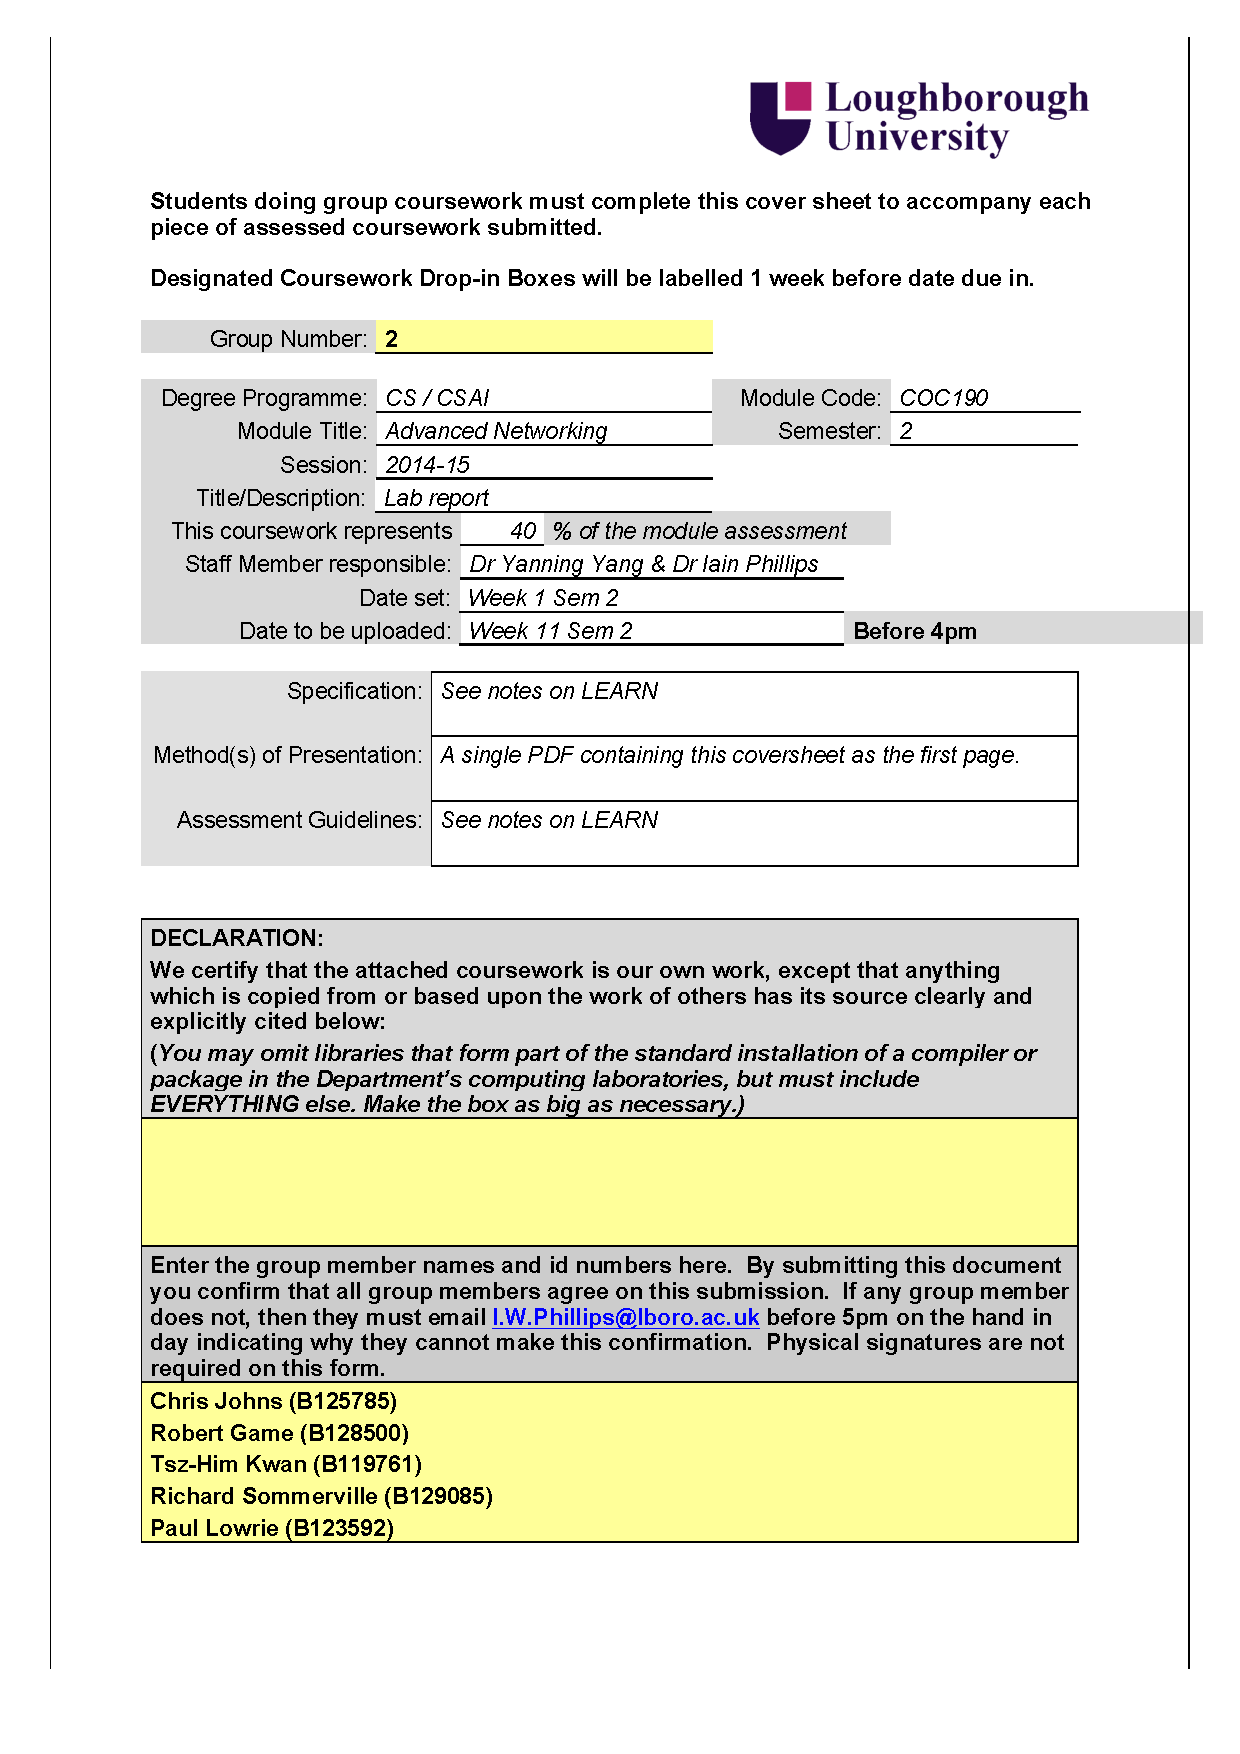
\includepdf[pages={1}]{coversheet.pdf}
\maketitle

\tableofcontents

\chapter{Network Design}
\section{Topology}
\section{Address Allocation}
\subsection{IPv4}
\subsection{IPv6}

\chapter{Network Diagram}
\section{IPv4}
\section{IPv6}

\chapter{Router Configuration}
\section{Static Routing}
\section{Interior Dynamic Routing}
\section{Security}
\section{Interdomain Routing}

\chapter{Laptop Configuration}
\section{DNS}
DNS is configured for the entire \texttt{8.0.0.0/24} block using the 
\texttt{.group2} domain. The three DNS servers: \texttt{ns1.group2}, \texttt
{ns2.group2} and \texttt{ns3.group2} are arranged to provide redundancy. \texttt
{ns1} is hosted on the laptop connected to \texttt{Alpha} and operates as the
master nameserver. \texttt{ns2} and \texttt{ns3} are configured as slaves to the
\texttt{ns1} master.
\begin{lstlisting}[caption={Master \texttt{named.conf.options}},label=
{listing:master-dns-named-conf-options}]
options {
        directory "/var/cache/bind";

        recursion yes;
        allow-recursion { any; };
        allow-query { any; };
        allow-transfer { 12.0.2.2; 12.0.3.2; };

        forwarders {
                10.2.2.1;
        };
};
\end{lstlisting}
\begin{lstlisting}[caption={Master \texttt{named.conf.local}},label=
{listing:master-dns-named-conf-local}]
zone "group2" {
    type master;
    file "/etc/bind/zones/db.group2";
    allow-transfer { 12.0.2.2; 12.0.3.2; };
};
zone "12.in-addr.arpa" {
    type master;
    file "/etc/bind/zones/db.12";
    allow-transfer { 12.0.2.2; 12.0.3.2; };
};
\end{lstlisting}
\begin{lstlisting}[caption={Master \texttt{db.group2}, for forward DNS},label=
{listing:master-dns-db-group2}]
$TTL    604800
@       IN      SOA     group2. admin.group2. (
                              2         ; Serial
                         604800         ; Refresh
                          86400         ; Retry
                        2419200         ; Expire
                         604800 )       ; Negative Cache TTL
;
; name servers - NS records
                IN      NS      ns1.group2.
                IN      NS      ns2.group2.
; name servers - A records
ns1.group2.     IN      A       12.0.1.2
ns2.group2.     IN      A       12.0.2.2

; 12.0.0.0/8 - A records
alpha.group2.   IN      A      12.1.1.1
bravo.group2.   IN      A      12.2.2.2
charlie.group2. IN      A      12.3.3.3
\end{lstlisting}
\begin{lstlisting}[caption={Master \texttt{db.12}, for reverse DNS},label=
{listing:master-dns-db-12}]
$TTL    604800
@       IN      SOA     group2. admin.group2. (
                              3         ; Serial
                         604800         ; Refresh
                          86400         ; Retry
                        2419200         ; Expire
                         604800 )       ; Negative Cache TTL
; name servers
        IN      NS      ns1.group2.
        IN      NS      ns2.group2.

; PTR Records
2.1.0   IN      PTR     ns1.group2.    ; 12.0.1.2
2.2.0   IN      PTR     ns2.group2.    ; 12.0.2.2
1.1.1   IN      PTR     alpha.group2.  ; 12.1.1.1
2.2.2   IN      PTR     bravo.group2.  ; 12.2.2.2
3.3.3   IN      PTR     charlie.group2.  ; 12.3.3.3
\end{lstlisting}
\begin{lstlisting}[caption={Slave \texttt{named.conf.options}},label=
{listing:slave-dns-named-conf-options}]
options {
        directory "/var/cache/bind";

        recursion yes;
        allow-recursion { any; };
        allow-query { any; };
        allow-transfer { none; };

        forwarders {
                10.2.2.1;
        };
};
\end{lstlisting}
\begin{lstlisting}[caption={Slave \texttt{named.conf.local}},label=
{listing:slave-named-conf-local}]
zone "group2" {
    type slave;
    file "db.group2";
    masters { 12.0.1.2 };
};

zone "12.in-addr.arpa" {
    type slave;
    file "db.12";
    masters { 12.0.1.2 };
};
\end{lstlisting}

\section{Webserver}
\section{Configuration Backups}
\section{Email}

\end{document}